

To evaluate the extraction framework, a manually annotated event-level evaluation dataset was constructed. All articles in this dataset describe realised drought impacts in the Netherlands, allowing the evaluation to focus exclusively on extraction performance rather than article relevance.

The dataset was created by manually annotating all drought impact events within each article. Every event consists of a reported location together with its associated impact category, severity, temporal recency, and supporting evidence. Model predictions are compared against these manually created annotations to evaluate extraction quality.

The dataset was constructed using an iterative sampling procedure to ensure broad coverage of drought impact types. Articles were manually reviewed and annotated until sufficient coverage of the impact taxonomy was achieved, resulting in a dataset containing at least ten distinct drought impact categories. All annotations were performed using a custom Streamlit application developed specifically for this thesis, enabling efficient article review and event-level annotation.

\subsection{Evaluated Models}

Five commercially available Large Language Models (LLMs) were evaluated in this study: Claude 4.6 Sonnet, GPT-5.4 mini, Gemini 3.1 Pro, Gemini 3.5 Flash, and Gemini 3.1 Flash-Lite. These models were selected because they represent recent state-of-the-art models from three major providers and all support structured output through Pydantic schemas. This allows the same extraction framework to be evaluated across different model families without modifying the prompt or extraction pipeline.

The selected models span a wide range of performance characteristics and inference costs (Table~\ref{tab:evaluated_models}). The comparison includes both flagship models, which are designed to maximise language understanding and instruction following, and smaller models that prioritise inference speed and computational efficiency. This allows us to evaluate the trade-off between extraction quality and operational cost.

Flagship models, such as Claude 4.6 Sonnet and Gemini 3.1 Pro, generally contain more parameters and computational capacity. As a result, they are expected to perform better on complex language understanding tasks, such as identifying multiple drought events within a single article, interpreting indirect temporal expressions, distinguishing closely related impact categories, and consistently producing structured outputs. These models therefore provide an upper bound on the extraction performance that can currently be achieved. 

GPT-5.4 mini represents an intermediate model that aims to retain much of the reasoning ability of larger models while substantially reducing inference cost. The Gemini Flash models are designed for high-throughput applications, where low latency and low cost are prioritised over maximum reasoning performance. In particular, Gemini 3.1 Flash-Lite targets large-scale processing pipelines in which hundreds of thousands of documents must be analysed. Although these smaller models may sacrifice some extraction accuracy, their lower computational cost makes them attractive for constructing large drought impact databases. 

The goal of this comparison is not to determine which provider develops the strongest general-purpose language model. Instead, the models are evaluated under identical experimental conditions to determine which provides the best balance between extraction quality, structured output reliability, and computational cost for our news-archive corpus of 20k aritcle's. 

\begin{table}[h!]
\centering
\caption{Evaluated LLMs and inference costs (May 2026).}
\label{tab:evaluated_models}
\small
\begin{tabular}{llcc}
\hline
\textbf{Provider} & \textbf{Model} & \textbf{Input / 1M} & \textbf{Output / 1M} \\
\hline
Anthropic & Claude 4.6 Sonnet & \$3.00 & \$15.00 \\
OpenAI & GPT-5.4 mini & \$0.75 & \$4.50 \\
Google & Gemini 3.1 Pro & \$2.00 & \$12.00 \\
Google & Gemini 3.5 Flash & \$1.50 & \$9.00 \\
Google & Gemini 3.1 Flash-Lite & \$0.25 & \$1.50 \\
\hline
\end{tabular}
\end{table}

\subsection{Controlled Experimental Setup}

To ensure a fair comparison, all models were evaluated under identical experimental conditions. Every model received the same newspaper articles, the same system prompt, and the same Pydantic extraction schema described in Chapter~\ref{...}. No model-specific prompt engineering or parameter tuning was performed.

The preprocessing pipeline was identical for every experiment, ensuring that each model received the same input representation. Furthermore, all models were evaluated on the same manually annotated event-level evaluation dataset.

To minimise stochastic variation, the temperature was fixed at 0 for every model. Structured output validation was performed using Pydantic, and requests that failed schema validation were automatically retried. The LiteLLM library was used to provide a unified interface across all model providers.

The performance of each model was evaluated using event-level extraction metrics. The primary evaluation metric is the location-impact F1-score, which measures whether the model correctly identifies drought impacts together with their associated locations. An extracted event is considered correct when the predicted location and impact category match the manually annotated event. Precision, recall, and F1-score are calculated as:

\[
Precision = \frac{TP}{TP + FP}
\]

\[
Recall = \frac{TP}{TP + FN}
\]

\[
F1 = 2 \times \frac{Precision \times Recall}{Precision + Recall}
\]where $TP$ represents correctly extracted events, $FP$ represents incorrectly extracted events, and $FN$ represents missed events.

Additionally, a stricter location-impact-severity-recency F1-score is calculated. For this metric, an extracted event is considered correct only when the location, impact category, severity, and temporal recency match the manually annotated event. This metric evaluates the complete quality of the structured extraction and captures errors caused by incorrect attribute extraction.








\subsection{Final Evaluation Dataset}
\label{subsubsec:final_dataset}

The final evaluation dataset contains 65 newspaper articles and 33 manually annotated drought impact events, covering 10 of the 20 predefined drought impact categories. The dataset was designed to maximise coverage of impact types rather than reflect the true distribution of drought impacts in the Netherlands.

Figure~\ref{fig:label_severity_recency_distributions} summarises the event-level distributions. Most impacts are classified as low or moderate severity, and most reported events occurred within one month of publication, reflecting the tendency of newspapers to report recent drought impacts.

\begin{figure}[h!]
\centering

\begin{minipage}{0.15\linewidth}
\centering
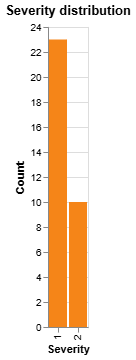
\includegraphics[width=\linewidth]{figures/severity_distribution.png}
\caption*{(a) Severity}
\end{minipage}
\hfill
\begin{minipage}{0.15\linewidth}
\centering
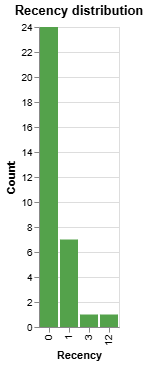
\includegraphics[width=\linewidth]{figures/recency_distribution.png}
\caption*{(b) Recency}
\end{minipage}
\hfill
\begin{minipage}{0.65\linewidth}
\centering
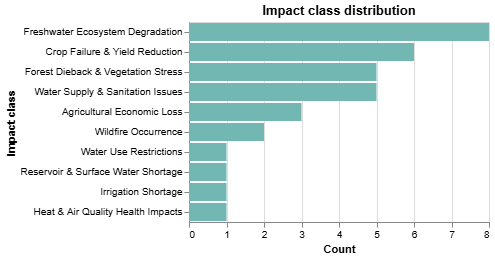
\includegraphics[width=\linewidth]{figures/impact_class_distribution.png}
\caption*{(c) Impact categories}
\end{minipage}

\caption{Distribution of event-level attributes and impact categories in the evaluation dataset.}
\label{fig:label_severity_recency_distributions}
\end{figure}

The impact category distribution is uneven, with agriculture, water resources, ecosystems, and forest-related impacts occurring most frequently. This reflects both newspaper reporting patterns and the event definition used in this study. Articles often describe the same type of impact across multiple locations, resulting in multiple annotated events within a single impact category. For example, a single article describing freshwater ecosystem degradation across several municipalities will produce multiple events, as each affected location is annotated separately. One single article has the potential to skew this entire distribution. Although the dataset does not provide equal representation across all impact categories, it contains sufficient diversity to compare LLM extraction performance.